
\documentclass[12pt,a4paper]{scrartcl}

\usepackage[a4paper, left=2cm, right=1cm, bottom=1cm, top=1cm, includeheadfoot]{geometry}
\usepackage[ngerman]{babel}
\usepackage[utf8]{inputenc} % comment this if you uncomment utf8x
%\usepackage[utf8x]{inputenc} % uncomment this if there are problems with 'ä', 'ü', 'ö'
\usepackage{ucs}
\usepackage[usenames,dvipsnames]{xcolor}
\usepackage[fleqn]{amsmath}
\usepackage{amsfonts}
\usepackage{amssymb}
\usepackage{color}
\usepackage{listings}
\usepackage{hyperref}
\usepackage{amsfonts}
\usepackage{listings}
\usepackage{scrpage2}
\usepackage{graphicx}


\definecolor{mygray}{rgb}{0.9,0.9,0.9}
\lstset{language=[Visual]Basic, morekeywords={param, local}}


\lstset{
   literate={ö}{{\"o}}1
           {ä}{{\"a}}1
           {ü}{{\"u}}1
           {ß}{{\ss}}1
           {é}{{\'e}}1,
   inputencoding=ansinew,
   extendedchars=true,
   basicstyle=\scriptsize\ttfamily,
   numberstyle=\scriptsize,
   breaklines=true,
   tabsize=2,
   numbersep=5pt
}
\lstdefinestyle{customcpp}{
   language=C++,
   backgroundcolor=\color{mygray},
   numbers=left,
   keywordstyle=\color{blue}\bfseries,
   stringstyle=\color{BrickRed}\ttfamily,
   commentstyle=\color{OliveGreen}\ttfamily,
   showspaces=false,
   showstringspaces=false,
   showtabs=false
}
\lstdefinestyle{customoutput}{
   backgroundcolor=\color{mygray},
   numbers=none,
   showspaces=false,
   showtabs=false
}

\newcommand{\sourceCode}[1]{\lstinputlisting[style=customcpp]{#1}} %beinhaltet alle benötigten Packages etc.
\begin{document}
\graphicspath{{./}}

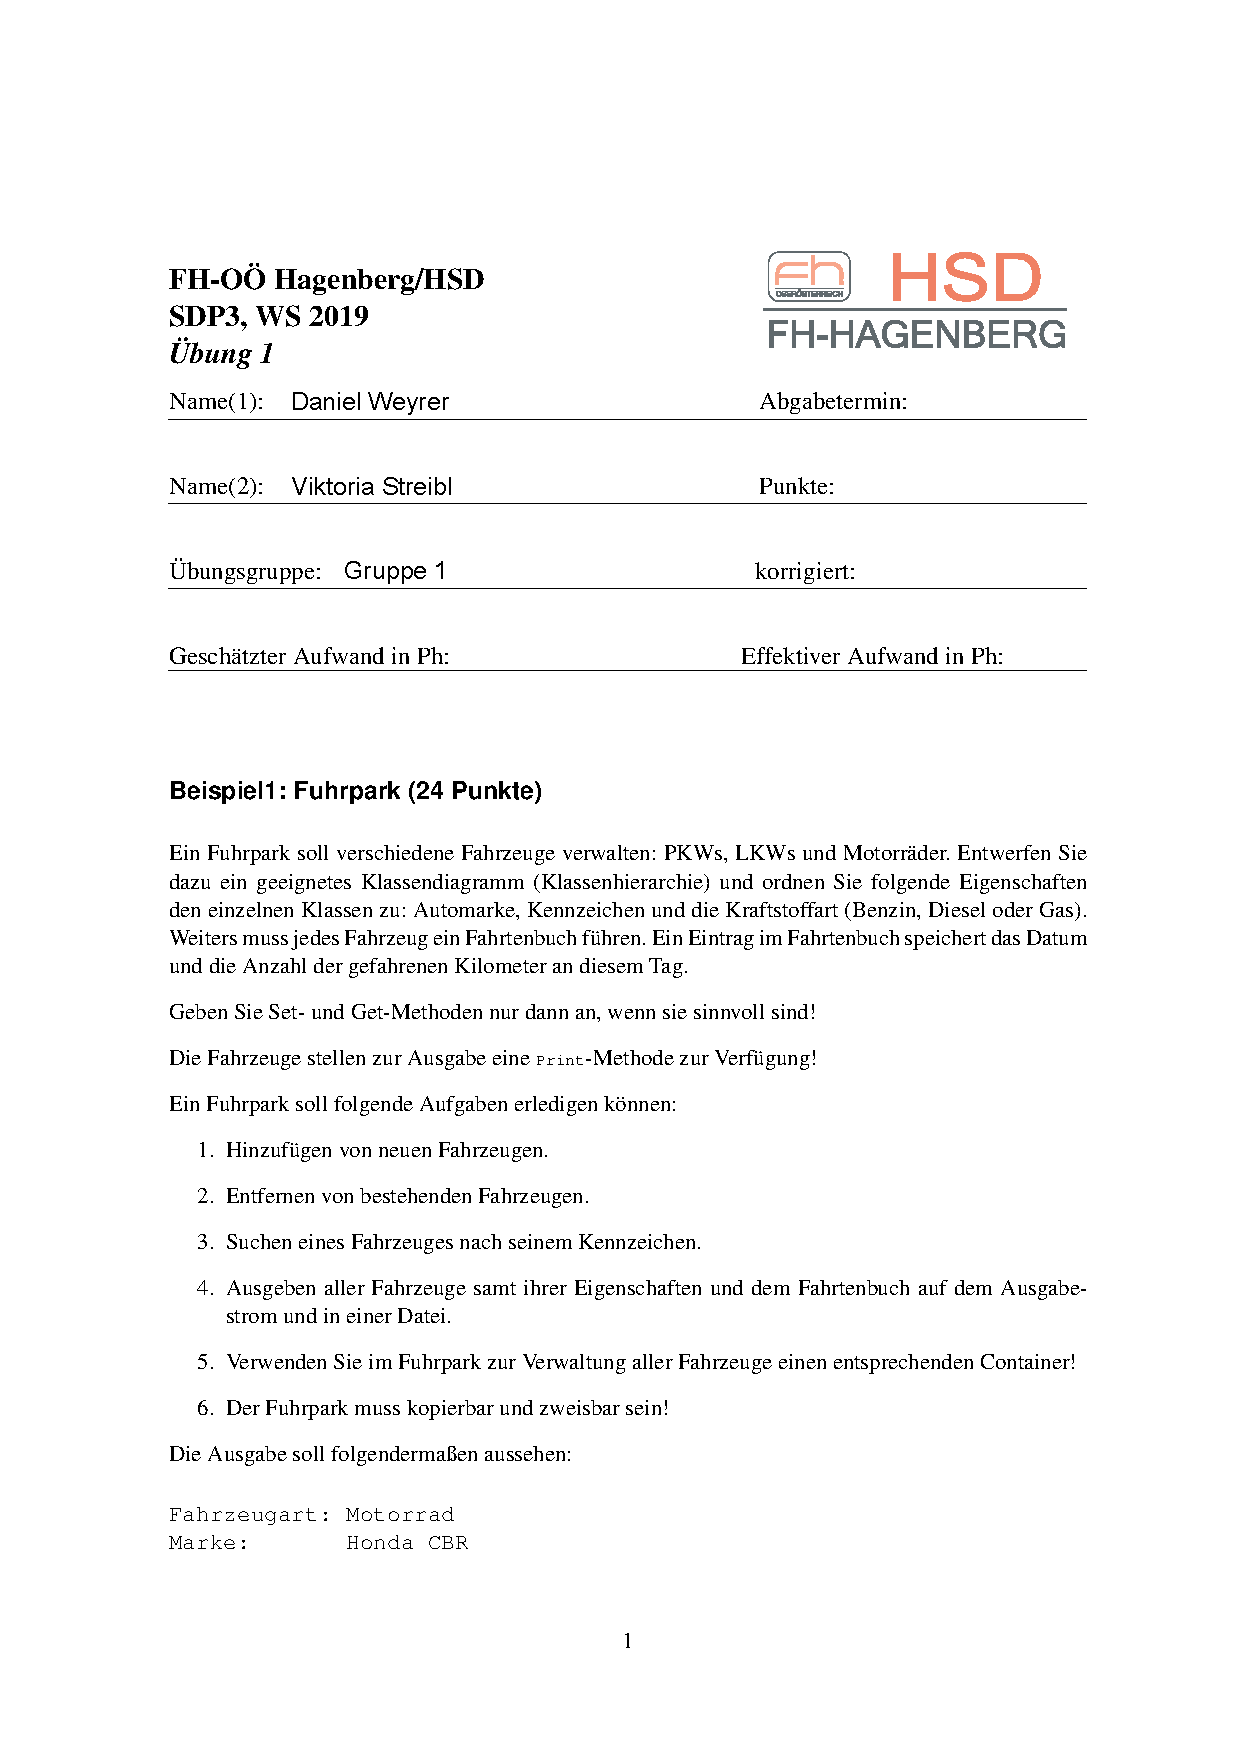
\includepdf[pages=-]{Angabe.pdf}

\title{SDP - Exercise 01} % Übungsname und Nummer angeben
\subtitle{winter semester 2019/20} % Semester angeben oder auskommentieren, falls nicht erwünscht
\author{
Viktoria Streibl - S1810306013\\
  Daniel Weyrer - S1820306044
} % Autorenname
\date{\today} % Das heutige Datum automatisch einfügen

\maketitle % Titelseite erstellen

\newpage
\tableofcontents % Inhaltsverzeichnis erstellen
\newpage

\section{Organizational}
\subsection{Team}
\begin{itemize}
	\item Viktoria 	Streibl 		- 	S1810306013
	\item Daniel 	Weyrer		-	S1820306044
\end{itemize}

\subsection{Roles and responsibilities}

\subsubsection{Jointly}
\begin{itemize}
	\item planning
	\item testing (Testdriver)
	\item Documentation
	\item Systemdocumentation
	\item Class Diagram
\end{itemize}

\subsubsection{Viktoria Streibl}
\begin{itemize}
	\item Base Class for Vehicles
	\item Derived Classes
		\subitem Class Motorcycle
		\subitem Class Car
		\subitem Class Truck
	\item Class Logbook
		\subitem plausibility test of input data (current Mileage and Date)
\end{itemize}

\subsubsection{Daniel Weyrer}
\begin{itemize}
	\item Main Class Carpool
\end{itemize}

\subsection{Effort}

\subsubsection {Viktoria Streibl}
\begin{itemize}
	\item estimated: 7ph 
	\item actually: 10 ph
\end{itemize}

\subsubsection {Daniel Weyrer}
\begin{itemize}
	\item estimated: 6ph 
	\item actually: 8 ph
\end{itemize}

\section{Requirenment Definition(System Specification)}
It was a carpool desired the various types of vehicles includes, such as cars, trucks and motorcycles. Each vehicle type should also include and output some key data such as car make, license plate and fuel type. In addition, each vehicle must keep a logbook and enter the kilometers driven in one day.
Any number of vehicles can be added and deleted in the program. You can search for the license plate and output all vehicles with the basic data.

\section{System Design}
\subsection{Classdiagram}
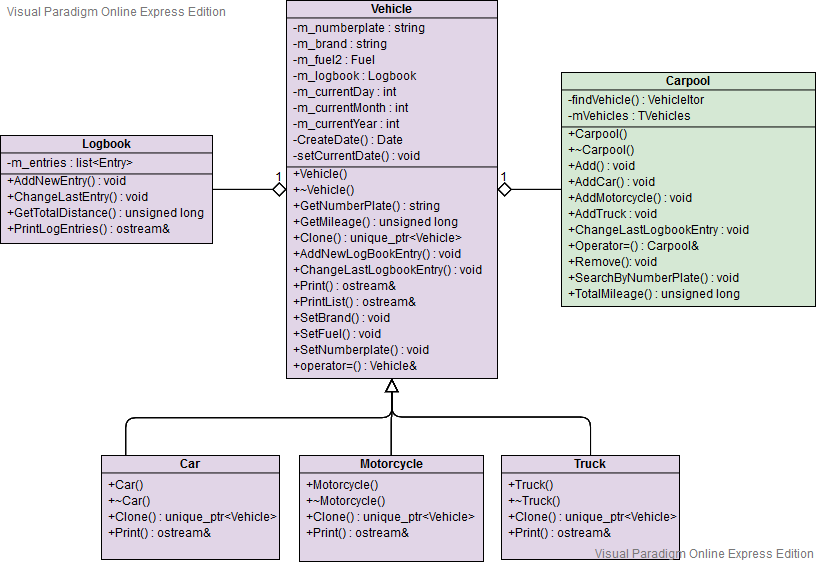
\includegraphics[scale=0.65]{ClassDiagram}

\subsection{Design Decisions}
\subsubsection{Inheritance}
The program should output the type of vehicle. To implement this as simple as possible, a base class has been implemented which contains all common functions and variables. A function "Print" is overloaded in the classes the heirs and there immediately the correct type is spent.
Furthermore, this approach allows a quick expansion of other vehicle types.

\subsubsection{Fuel}
The Fuel was declared as enum. You can also expand this easily and it is uniform.

\subsubsection{Search Vehicle}
Vehicle is searched by vehicle number because it has to be unique. This is already regulated by the authority, which is why we do not check it it is unique.

\subsubsection{Logbook}
The logbook contains a date and a mileage of the respective day. This date is stored in a stuct to check if the day, month and year is available.
If the date of a new entry is older than the date of the last entry, an error message will be displayed. Only current entries can be entered. If new entry is the same date as the old entry, then the mileage will be added up.

\section{Component Design}
\subsection{Class Carpool}
Manages all vehicles in the carpool.
It contains the following functions:
\begin{itemize}
	\item Add a new Vehicle
	\item Remove a Vehicle
	\item Add new logbook entry
	\item Change last logbook entry
	\item Search vehicle by numberplate
	\item Print all vehicles
	\item Get the sum of milages
\end{itemize}

The Carpool class manages all Verhicles. It uses unique pointers stored in a vector, to avoid shallow-copies.
With the methods "AddCar", "AddTruck" and "AddMotorcycle" a new vehicle can be created. Should a car already exist with the same license plate. So this vehicle is not stored and an error message output.
"Remove" deletes a vehicle with a specific flag. If none is stored with the license plate an exception get`s thrown and caught in the same method.
With "AddLogbookEntry" a day, month, year and the driven kilometers are given and saved as a new entry in the logbook.
With "ChangeLastLogbookEntry" the last entry can be edited.
With the method "SearchByNumberplate" it is possible to search for a vehicle with the specific flag and to output it.
"PrintVehicles" outputs all stored vehicles, more exactly in the respective classes.
"TotalMileage" provides the total number of kilometers driven, driven by all vehicles.

\subsection{Class Vehicle}
Is the base class of all vehicle types.
It contains the following functions:
\begin{itemize}
	\item Add Brand
	\item Add Numberplate
	\item Add Fuel
	\item Add new logbook entry
	\item Change last logbook entry
	\item Get numberplate
	\item Get driven kilometers
\end{itemize}

Vehicle is the base class of all vehicle types. It contains the brand, numberplate and fuel of a vehicle.
Furthermore, it also manages the logbook entries of a single vehicle.
There is a setter for brand, numberplate and fuel. For numerplate and the kilometers driven is also a getter.
With "AddLogbookEntry" a day, month, year and the driven kilometers are given and saved as a new entry in the logbook.
With "ChangeLastLogbookEntry" the last entry can be edited.

The private methode "CreateDate" converts the individual values of day, month and year to a struct named "Date".
It also checks if the day is between 1 and 31. But not how many days in a month. That was
not considered for this solution. Thus, a 30th February is possible as a date.
The month also checks if it is between 1 and 12 and if the year is not negative.
Another check is made if the date is not in the future. Which is why the private method "setCurrentDate" saves the current date, so it
is able to compare later.

\subsection{Class Car}
This class represents a car.
\begin{itemize}
	\item Print all car data and the associated log entries
\end{itemize}

"Print" overrides the function of the base clase and outputs the vehicle type: "PKW", as well as brand and numberplate.
Further, all logbook entries will be read out and printed out.

\subsection{Class Truck}
This class represents a truck.
\begin{itemize}
	\item Print all truck data and the associated log entries
\end{itemize}

"Print" overrides the function of the base clase and outputs the vehicle type: "LKW", as well as brand and numberplate.
Further, all logbook entries will be read out and printed out.

\subsection{Class Motorcycle}
This class represents a motorcycle.
\begin{itemize}
	\item Print all motorcycle data and the associated log entries
\end{itemize}

"Print" overrides the function of the base clase and outputs the vehicle type: "Motorrad", as well as brand and numberplate.
Further, all logbook entries will be read out and printed out.

\subsection{Class Logbook}
Class for collection driver data. It saves the driven kilometer per day of a vehicle.
It contains the following functions:
\begin{itemize}
	\item Add new logbook entry
	\item Change last logbook entry
	\item Print all logbook entries
	\item Adds up all the kilometers together
\end{itemize}

This class has a struct "Date" that includes the current date with "Tag", "Monat" and year "Jahr". It saves the entries in a list. An entry consists of two parts, a date and the kilometers driven on this day. AddNewEntry adds a new entry to the list. However, if the new date is older than the last entry, so an error is advertised. If a new entry has the same date as that of the last one, the two mileage become added and written to the list. With "ChangeLastEntry" you can change the last saved entry. "GetTotalDistance" counts the kilometers that have been saved in Logbook and returns them.

\subsection{TestDriver}
The Testdriver test alle functions of the Carpool. It adds cars, trucks and motorcycles and deletes them.
It searchs vehicles by numerplate and print all of them. It tests all logbook functions and the carpool.

\section{Test Protocol}
It has been tested in the file "TestDriver", the following points have been tested:
\begin{itemize}
	\item Add new vehicle
	\item Remove vehicle
	\item Find a vehicle
	\item Print vehicles
	\item Test Logbook
	\item Test Carpool
\end{itemize}

\subsection{Console Output}
\sourceCode{./Carpool/output.txt}

\section{Source Code}

\subsection{Class Carpool}
\subsubsection{Carpool.h}
\sourceCode{./Carpool/Carpool/Carpool.h}
\subsubsection{Carpool.cpp}
\sourceCode{./Carpool/Carpool/Carpool.cpp}

\subsection{Class Vehicle}
\subsubsection{Vehicle.h}
\sourceCode{./Carpool/Carpool/Vehicle.h}
\subsubsection{Vehicle.cpp}
\sourceCode{./Carpool/Carpool/Vehicle.cpp}

\subsection{Class Logbook}
\subsubsection{Logbook.h}
\sourceCode{./Carpool/Carpool/Logbook.h}
\subsubsection{Logbook.cpp}
\sourceCode{./Carpool/Carpool/Logbook.cpp}

\subsection{Class Motorcycle}
\subsubsection{Motorcycle.h}
\sourceCode{./Carpool/Carpool/Motorcycle.h}
\subsubsection{Motorcycle.cpp}
\sourceCode{./Carpool/Carpool/Motorcycle.cpp}

\subsection{Class Car}
\subsubsection{Car.h}
\sourceCode{./Carpool/Carpool/Car.h}
\subsubsection{Car.cpp}
\sourceCode{./Carpool/Carpool/Car.cpp}

\subsection{Class Truck}
\subsubsection{Truck.h}
\sourceCode{./Carpool/Carpool/Truck.h}
\subsubsection{Truck.cpp}
\sourceCode{./Carpool/Carpool/Truck.cpp}

% Um Quellcode einzufügen einfach diesen Befehl verwenden:
%\sourceCode{Relativer/Pfad/zum/SourceCode.Endung}

\end{document}